% Place after \appendix in the one-column manuscript. The inventory uses xltabular, ragged2e, array, and booktabs.
\section{Statistical methods and validation protocols}
\label{app:statistical-methods}
\label{app:statmethods}
\label{app:methods}

\subsection{Covariance construction}
\label{app:covariance-construction}
\label{sec:variance}
\label{sec:combine}
\label{sec:seedscan}
\label{sec:bootstrap}
\label{app:poisson}
\label{sec:universes}
\label{app:pair}
\label{sec:minerva}

The two-dimensional covariance $Q_R$ in Eq.~\eqref{eq:muon-covariance-block-sum} is evaluated on the \lrval{q-ncells} reported cross-section densities. Each ensemble uses the same five-iteration procedure as the central value, with the input varied according to the source under study. The block sum neglects cross-covariances between sources and assumes that the changes from simultaneous input variations are additive. In particular, the statistical and systematic blocks use a fixed training seed, so their variation with the choice of seed is outside the block sum.

\paragraph{Statistical and training-seed blocks.} The statistical bootstrap draws independent Poisson weights of mean one for each event in data, signal simulation, and background simulation. Each simulated signal event receives a single draw shared by its truth and reconstruction records. These factors are propagated through the full unfolding, including the background treatment and the cross-section extraction. Independent Poisson counts are the large-sample limit of the multinomial bootstrap counts for any fixed subset of events. For $N=300$ replicas $X^{(k)}$ at the central training seed, the covariance is
\begin{equation}
  \begin{aligned}
    \overline X &= \frac{1}{N}\sum_{k=1}^{N}X^{(k)},\\
    C_{\mathrm{stat}} &= \frac{1}{N-1}\sum_{k=1}^{N}
     (X^{(k)}-\overline X)(X^{(k)}-\overline X)^{\mathsf T} .
  \end{aligned}
  % amsmath defers one label per display. Use the label writer directly for aliases.
  \expandafter\let\expandafter\label\csname ltx@label\endcsname
  \label{eq:app-bootstrap-covariance}
  \label{eq:bootcov}
\end{equation}
Centering on $\overline X$ leaves its displacement from the central value out of the covariance. The displacement is a median of 0.25 statistical standard deviations across bins and measures the bootstrap offset. Its relation to bias relative to truth remains undetermined.

The training-seed block uses the first 20 of the statistical block's bootstrap replicas at each of five settings of the random seeds for the two classifiers and the missed-event regressor. We average the unfolded vectors over the 20 replicas at each setting and take the sample covariance of the five averages, using Eq.~\eqref{eq:app-bootstrap-covariance} with $N=5$. Matching the replicas isolates seed dependence on common inputs, with a contribution from the bootstrap--seed interaction remaining in the means at the $1/20$ variance scale. The block has rank at most four.

\paragraph{Systematic universes.} Each universe propagates its truth and reconstructed weights through an unfolding matched to the nominal calculation in training settings and event processing. Missed signal events carry the universe's truth weights, and lateral variations, which change reconstructed kinematics, use the event selection for the varied simulation. This changes which simulated events enter the reconstructed sample and which enter the missed-event correction. The flux affects both the simulated event weights and the denominator in Eq.~\eqref{eq:flux-averaged-cross-section}. For each flux universe we divide the unfolded yields by the integrated flux with the same universe index. The MINOS muon-energy-scale variations likewise use their own flux normalizations, which carry the correlated flux response. Adding a separate flux--MINOS cross term would count that effect twice. The three GEANT hadron-interaction bands follow the MAT-MINERvA treatment at our pinned commit, which reweights only reconstructed events and leaves the efficiency denominator unchanged. The current MAT-MINERvA release also reweights the denominator. Each lateral band of the quoted universe block uses a single unfold at the central training seed, so it includes that seed's training noise.

With $X^{(b,u)}$ the result in universe $u$ of band $b$ and $a_{bu}$ its normalized weight, the MINERvA Analysis Toolkit convention gives
\begin{equation}
  \begin{aligned}
    \overline X_b &= \sum_u a_{bu} X^{(b,u)}, \qquad \sum_u a_{bu}=1, \\
    C_b &= \sum_u a_{bu}(X^{(b,u)}-\overline X_b)
                     (X^{(b,u)}-\overline X_b)^{\mathsf T} .
  \end{aligned}
  \expandafter\let\expandafter\label\csname ltx@label\endcsname
  \label{eq:app-universe-covariance}
  \label{eq:matcov}
\end{equation}
Centering each band on its universe mean excludes the offset of that mean from the central value. The population normalization factors are $1/N_b$ for a band with $N_b$ equally weighted universes. For the 100 flux universes, they incorporate the neutrino--electron scattering and inverse-muon-decay constraints. For a symmetric two-universe band, Eq.~\eqref{eq:app-universe-covariance} is the outer product of half the difference of the two results. Using their nominal value as the center instead would add the outer product of their mean offset. This distinction matters when the unfolding responds asymmetrically to the two shifts.

The systematic sweep contains 187 universes in 44 bands. The covariance sums 43 bands after removing a duplicated nonresonant-pion variation. The target normalization is added as the fully correlated term
\begin{equation}
  (0.014X_0)(0.014X_0)^{\mathsf T},
  \label{eq:normband}
\end{equation}
where $X_0$ is the central vector. The per-band aggregation follows that of the published measurement, with the same population normalization for both the two-universe bands and the flux multisim~\cite{MINERvA:2021owq}. An elementwise comparison with the toolkit for identical universe vectors checks the aggregation convention separately from the propagation of the weights through the unfolding.

\paragraph{Run-period and prior-shape terms.} The run-period term uses three separately unfolded groups. For each group we divide the unfolded result bin by bin by that group's simulated truth, subtract the exposure-weighted mean of the three ratios, and multiply the resulting deviations by the pooled central cross section. The covariance is formed from the outer products of these three displacement vectors about that reference. The same construction is used on the sixteen-cell integrals, scaling the ratio deviations to the pooled integrals to propagate correlated changes across cells. The resulting matrices have rank at most two. The spread includes the finite statistics of the individual periods, with no subtraction for their sampling noise. The construction was chosen after the period differences were observed (Appendix~\ref{app:choices-after-results}).

For prior-shape sensitivity, the simulation prior is reweighted in turn using the shapes of GENIE with Valencia MEC, NuWro, and GiBUU relative to nominal GENIE, and the data are unfolded again. If $s_g$ is the resulting displacement from the central value for reweighting $g$, we form $C_{\mathrm{model}}=\sum_g s_gs_g^{\mathsf T}$, with no ensemble-size divisor. The reweightings preserve the prior's normalization. We give this term separately from $Q_R$ and include it in the sixteen-cell covariance [Eq.~\eqref{eq:sixteen-cell-covariance}]. It describes sensitivity to these shape changes and has no assigned sampling distribution.

\paragraph{Sixteen-cell covariance.} The sixteen-cell block $C_e$ combines a refitted statistical bootstrap with flux, interaction-model, detector, and lateral-band covariances and the correlated target normalization. The refit includes the negative-weight background refinement. Training is deterministic in this configuration, so the seed term is zero. The response block $C_{\mathrm{resp}}$ is a sum of four outer products. For each deposit category (protons, mesons, electromagnetic showers, and other deposits), the vector is half the difference between the unfolded results after shifting that category's reconstructed energy up and down by one standard deviation. These shifts are made separately and their outer products are added to $C_e+C_{\mathrm{model}}$ and the run-period term as specified in Eq.~\eqref{eq:sixteen-cell-covariance}. We form the component matrices in the space of cell integrals. In particular, the response vector for a deposit category is obtained by aggregating each shifted unfolding to the sixteen regions before taking the half-difference. This retains correlations among regions and permits coherent propagation to sums of cells. For a generator comparison we add the prediction's diagonal finite-sample covariance, with entries given by the sum of squared event weights in each region after converting the weights to cross-section units.

\subsection{Numerical conventions, inversion, and rank}
\label{app:covariance-inversion}
\label{sec:invert}
\label{sec:rank}
\label{sec:nd-declarations}

We use Cholesky factorization to solve systems with a positive-definite covariance. When checking a sample covariance for numerical definiteness, a failure attributable to roundoff can be probed by adding $\epsilon I$, with $\epsilon=10^{-12}\operatorname{tr}(C)/n$ for an $n\times n$ matrix. This perturbation addresses numerical factorization. A covariance estimated from $N$ centered replicas has rank at most $\min(n,N-1)$ regardless of the factorization, and $N>n$ only permits full rank.

For the comparison with the published two-dimensional result, we use the Moore--Penrose inverse from a singular-value decomposition $C=U\operatorname{diag}(\sigma_i)V^{\mathsf T}$. In $C^+=V\operatorname{diag}(h_i)U^{\mathsf T}$, $h_i=1/\sigma_i$ for $\sigma_i>10^{-15}\sigma_{\max}$ and $h_i=0$ otherwise. For rank and conditioning diagnostics we instead use the eigenvalues of $(C+C^{\mathsf T})/2$. We count positive modes above $10^{-12}\lambda_{\max}$ (or the explicitly indicated cutoff), and quote the ratio of $\lambda_{\max}$ to the smallest retained eigenvalue.

Formally full rank can still leave the two-dimensional distance dominated by poorly determined modes. The universe covariance retains 138 of 205 modes at $10^{-12}\lambda_{\max}$, and adding the bootstrap raises that count to 205 with a retained condition number of $7.95\times10^{11}$. For $Q_R$ the count is 198 at $10^{-10}\lambda_{\max}$. The direct inverse of $Q_R$ gives a quadratic distance of 21.96 per reported bin against the published central value, compared with \chiPaperOurEdges{} using the published covariance on the same $p_T$ edges. The latter has a nearly diagonal, full-rank statistical block that provides variance in all directions. For numerical comparisons based on $Q_R$ alone, the truncated inverse uses the positive modes above $10^{-10}\lambda_{\max}$. In that convention the distance is the sum of squared residual amplitudes along the retained eigenvectors divided by their eigenvalues. Discarding directions changes the residual being tested, so the cutoff is part of the definition of the statistic. The publication comparison instead quotes the number of reported bins as the denominator, as specified in Appendix~\ref{app:comparison-closure-coverage}.

A multidimensional quadratic distance is quoted with its covariance, inverse and cutoff, retained rank, and sensitivity to rank truncation. The retained rank is the dimension of the statistic. In particular, projection cannot increase the rank of a covariance. For each sample covariance used in an inverse one must also specify its ensemble size and normalization, the inverted dimension, and any correction for finite-ensemble bias. For $N$ independent Gaussian draws and a fixed $p$-dimensional subspace, the inverse-bias factor is $(N-p-2)/(N-1)$ with $1/(N-1)$ covariance normalization, or $(N-p-2)/N$ with $1/N$ normalization, for $N>p+2$. These assumptions limit its use for a sum of systematic bands or a subspace selected from the same covariance spectrum. The sum of mean-centered band covariances has rank at most the sum of the individual ranks, and each band contributes at most $N_b-1$ independent directions. An independent normalization outer product can add at most one direction.

For multidimensional difference tests the rank cut is fixed before the outcome is read. In the sixteen-cell generator comparisons the quoted dimensions are 16 for the total statistic and 15 for the shape statistic, or \fvval{g-gibuu-total-ndf} and \fvval{g-gibuu-shape_only-ndf} on the restricted GiBUU domain. The joint tests in Appendix~\ref{app:joint-generator-tests} use an empirically calibrated statistic with a separate, shrinkage-based metric.

\subsection{Comparison statistics and closure}
\label{app:comparison-closure-coverage}
\label{sec:compare}
\label{sec:205bins}
\label{sec:chisq}
\label{sec:pull}
\label{sec:shape}
\label{sec:closure}
\label{sec:closure-tr}
\label{sec:closure-hv}
\label{sec:closure-alt}
\label{sec:assemble}

Let $K$ denote the cross-covariance between the OmniFold and published results. The covariance of their bin-by-bin difference $\Delta$ is
\begin{equation}
  \operatorname{Cov}(\Delta)=Q_R+V_{\mathrm{pub}}-K-K^{\mathsf T} .
  \label{eq:muon-difference-covariance}
\end{equation}
The sum $Q_R+V_{\mathrm{pub}}$ gives a distance per bin of \chiCombined{}. It omits the cross terms and counts shared uncertainties twice.

The two-dimensional comparison uses the 205 positive published bins on the $14\times16$ muon grid. We form $\Delta=X-X_{\mathrm{pub}}$ and quote
\begin{equation}
  \Delta^{\mathsf T}C^+\Delta/205
  \label{eq:chi2}
\end{equation}
and $\Delta_i/\sqrt{C_{ii}}$, using either the published covariance alone or its sum with $Q_R$. These are descriptive distances because the cross-covariance from the shared data and systematics is unavailable [Eq.~\eqref{eq:muon-difference-covariance}]. Removing the published statistical block from the sum changes the quadratic distance per bin from \chiCombined{} to \chiCombinedSubStat{} and still leaves the cross-covariance unknown. For the logarithmic distance we take the log of the binwise ratio and divide the summed covariance element $ij$ by $X_{\mathrm{pub},i}X_{\mathrm{pub},j}$.

To compare shapes, let $a$ be the bin-area vector and normalize $x$ to $s=x/(a^{\mathsf T}x)$. The Jacobian is
\begin{equation}
  J(x)=\frac{I-sa^{\mathsf T}}{a^{\mathsf T}x},\qquad
  C_s=JCJ^{\mathsf T} .
  \label{eq:app-shape-jacobian}
\end{equation}
For the shape diagnostic using the published covariance, $J$ is evaluated at the published central values. The unit-area constraint $a^{\mathsf T}s=1$ leaves at most 204 independent directions. For vectors of cell integrals, $a$ is the vector of ones. A rate-only comparison instead uses the squared difference of the two integrals divided by the variance $a^{\mathsf T}C a$.

Paired-replica comparisons propagate common input variations through both unfoldings and evaluate the difference. The covariance is estimated in the space of those differences, which incorporates the shared fluctuations in Eq.~\eqref{eq:muon-difference-covariance}. For the sixteen-cell comparison with binned IBU we propagate the statistical, weight-only systematic, and normalization terms and calibrate the quadratic distance on a simulated null of exact agreement. The comparison tests agreement between algorithms under those variations. Closure at known truth is assessed separately.

Signal-only closures compare the unfolded pseudo-data with a specified truth. In the two-dimensional truth-reweighting check, both the signal truth and its reconstructed counterpart are weighted by a function of true kinematics. The tested weights are $1+0.2\exp[-((p_T-0.4)/0.1)^2]$ and $1+0.1(p_\parallel-5)$, with momenta expressed in $\mathrm{GeV}/c$. The nominal simulation is used to unfold the pseudo-data. The score is the median absolute fractional residual over reported bins. A separate injected-feature score divides the residual by the size of the injection, following Ref.~\cite{Canelli:2025guide}. The higher-dimensional bump tests use the same truth-to-reconstruction weight transfer. Their recovery score is read on the one-dimensional projection of the deformed observable. The available-energy test applies a $30\%$ Gaussian enhancement centered at $0.3~\mathrm{GeV}$ with width $0.15~\mathrm{GeV}$. The injected change on the marginal is $18.1\%$, and the residual across 3D bins has a standard deviation of $3.2\%$. The $q_3$ test also uses Gaussian reweighting. The $W$ test applies a $30\%$ Gaussian enhancement centered at $1.23~\mathrm{GeV}$ with width $0.15~\mathrm{GeV}$. The ratio of the residual feature to the injected feature is graded in the peak bin, $1.1\leq W<1.4~\mathrm{GeV}$, where the residual is $4.2\%$ for a $23.1\%$ injection. Examining the individual $(E_{\mathrm{avail}},W)$ cells there reveals distortions that dilute in the $W$ projection.

In the hidden-variable check, reconstructed pseudo-data are multiplied by $1+A\exp[-((\Delta p_T-0.10)/0.05)^2]$, with $\Delta p_T$ in $\mathrm{GeV}/c$ and $A=0.05$, 0.10, or 0.30. The truth target is unchanged. Fitting the median signed fractional residual versus $A$ gives the leakage of the hidden resolution deformation into the unfolded muon distribution. The alternative-universe check instead uses pseudo-data from the positive quasielastic axial-mass variation or from one flux universe. Its reference is the nominal full-truth cross section multiplied binwise by the alternative-to-nominal ratio of accepted truth yields. This isolates recovery relative to a reference extrapolated with the nominal acceptance.

The sixteen-cell bias test scores the difference between the mean unfolded vector and the known truth. The scale is the reported covariance of an individual result, with the corresponding generator's outer product removed when the truth was derived from that generator. The prespecified criterion flags a truth for a quadratic distance with a $\chi^2_{\fvval{f0b-A7_genie_cv-n}}$ reference probability below \fvval{trig-p} or an absolute standardized mean residual above \fvval{trig-z} in any cell. Separate Poisson ensembles at held-out tunes probe the same bias criterion without drawing detector and interaction-model variations.

\subsubsection{Interval diagnostics for closure tests}
\label{app:closure-interval-diagnostics}

\paragraph{Two-dimensional closure at held-out tunes.} The 2D study draws the specified variations in \lrval{cov2d-ntoys} pseudo-experiments at each tune. The initial score uses the covariance rebuilt at that tune with the prior-shape term and without the run-period block. A bin is covered if its absolute residual is at most $\sqrt{C_{ii}}$. Joint containment uses
\begin{equation}
  \Delta_{\mathrm{true}}^{\mathsf T} C^+\Delta_{\mathrm{true}}
  \leq F^{-1}_{\chi^2_\nu}\!\bigl(2\Phi(1)-1\bigr),
  \label{eq:app-joint-coverage}
\end{equation}
where $\Phi$ is the standard normal cumulative distribution and $\nu$ is the retained rank. This quantile has the probability content of a Gaussian one-standard-deviation interval. A null simulation sets the minimum acceptable counts before the pseudo-experiment outcomes are read. We assess per-bin and joint counts separately. The counts in Sec.~\ref{sec:coverage-tunes} fall below the respective minima of \lrval{cov2d-ar23-kjoint} and \lrval{cov2d-g18-kjoint}.

The quadratic distance uses \lrval{cov2d-ar23-ndf} degrees of freedom at the first tune and \lrval{cov2d-g18-ndf} at the second. A descriptive check retaining only the \lrval{t2a-r1} or \lrval{t2a-r2} largest-variance directions also finds zero joint containments at each tune.

\begingroup
% Format the source's combined ranges as inequalities and percentage points.
\def\MuonCoverageCell#1--#2, #3--#4\relax{%
  $#1<p_T<#2\,\mathrm{GeV}/c$ and $#3<p_\parallel<#4\,\mathrm{GeV}/c$}
\def\MuonCoveragePoints#1--#2\relax{\fpeval{100*(#1)}--\fpeval{100*(#2)}}
The per-bin test flags \lrval{cov2d-ar23-nflagged} bins at the first tune and \lrval{cov2d-g18-nflagged} at the second, with the deficits attributed to bias in those bins. The bin with \expanded{\noexpand\MuonCoverageCell\lrval{cov2d-cell29-range}\noexpand\relax} is flagged at both tunes, with \lrval{cov2d-ar23-29-count} and \lrval{cov2d-g18-29-count} containments, respectively, against a threshold of \lrval{cov2d-ar23-29-kc}. The per-bin test resolves deficits in coverage of about \expanded{\noexpand\MuonCoveragePoints\lrval{cov2d-res-cell}\noexpand\relax} percentage points. The joint test scores the full residual vector and resolves a deficit of about \fpeval{100*\lrval{cov2d-res-joint}} percentage points. \par \endgroup

The intervals on data use $Q_R$ as defined in Eq.~\eqref{eq:muon-covariance-block-sum}.

\paragraph{Sixteen-cell closure at held-out tunes.} The study scores $C_{\mathrm{total}}$ with and without the neutron and proton transport bands. At both tunes the joint counts fall below the minimum of \fvval{ll5d-kjoint-all} for each variant. The response and run-period terms added for the $C_{\mathrm{rep}}$ regrade represent variations absent from the pseudo-experiments. The separate Poisson and noise-free mean-bias checks stay within their criteria at these tunes (Sec.~\ref{sec:closure-interval-diagnostics}). The joint interval shortfall leaves the relative contributions of bias and scatter unresolved.

\paragraph{Two-dimensional statistical intervals.}
\label{sec:coverage}
The quoted statistical block has had no coverage test. Appendix~\ref{app:choices-after-results} records the analysis choices for the earlier variant tested here.
% Search: coverage test of the quoted 2D statistical block (Q_R block, S1); held-out-MC re-test; KNOWN_ISSUES 85; statband-retest; coverage_fixed_truth/n2; COV2D; REGRADE (the primer's search at 0d919b1a, rerun; REGRADE-DECLARATION.md grades the COV2D toys against C_T + C_run(T), the full covariance, not the statistical block) @ caae27166e85

The fixed-truth coverage test of the earlier two-dimensional statistical band uses Poisson pseudo-data and scores the fractions within one and two band standard deviations of the fixed, unfluctuated truth. A band-to-scatter ratio between 0.9 and 1.1 under a Gaussian reference sets the prespecified windows $[\covTwoDWinOneLo,\covTwoDWinOneHi]$ and $[\covTwoDWinTwoLo,\covTwoDWinTwoHi]$. The score pools toy--bin containments. Coverage pooled over bins is not a simultaneous probability that every bin is covered. In \covTwoDNtoy{} pseudo-experiments the one-standard-deviation score is \covTwoDCOne{} and the two-standard-deviation score is \covTwoDCTwo{}. The latter falls below its acceptance window.

\phantomsection\label{sec:pull-diagnostic} In the separate same-ensemble diagnostic, we estimate each bin's standard deviation from the 200 unfolded replicas being scored and center each residual on the ensemble mean truth. The resulting fraction of standardized residuals within one standard deviation describes the ensemble's pull distribution. It is compared with the Gaussian probability of 0.6827.

\paragraph{Statistical intervals for the deterministic 5D purity control.}
\label{sec:coverage-5d}
The deterministic purity control fails the prespecified coverage futility rule at nominal truth and under an approximately $10\%$ reduction in signal rate with a weak $E_{\mathrm{avail}}$ slope. At the reduced rate, 51 of 153 cell, projection, and total integrals fail for the $68\%$ intervals, and 42 fail for the $95\%$ intervals (Fig.~\ref{fig:coverage-5d-paper}). The lowest empirical coverage for the $68\%$ intervals is 0.060. At nominal truth, two integrals fail for the $95\%$ intervals, with lowest coverage 0.850.

The end-to-end coverage assessment uses 400 pseudo-experiments per generated truth. It corrects each estimate by dividing by $1+\beta$, where $\beta$ is its relative nominal-truth bias, and combines the statistical standard deviation in quadrature with the corrected estimate times the standard error of $\beta$. It grades 153 integrals, retaining all 42 $(E_{\mathrm{avail}},W)$ cells, using separate Bonferroni adjustments over the integrals and three generated truths for each nominal coverage level. An integral fails if its upper confidence bound is below 0.66 for the $68\%$ interval or below 0.94 for the $95\%$ interval. The rate-reduced truth multiplies the signal by $1+0.2[E_{\mathrm{avail}}/(100\,\mathrm{GeV})-1/2]$ and keeps the background fixed. An invalid $q_3$ reweighting leaves the third generated truth outside the reported verdict.

\begin{figure}[H]
  \centering
  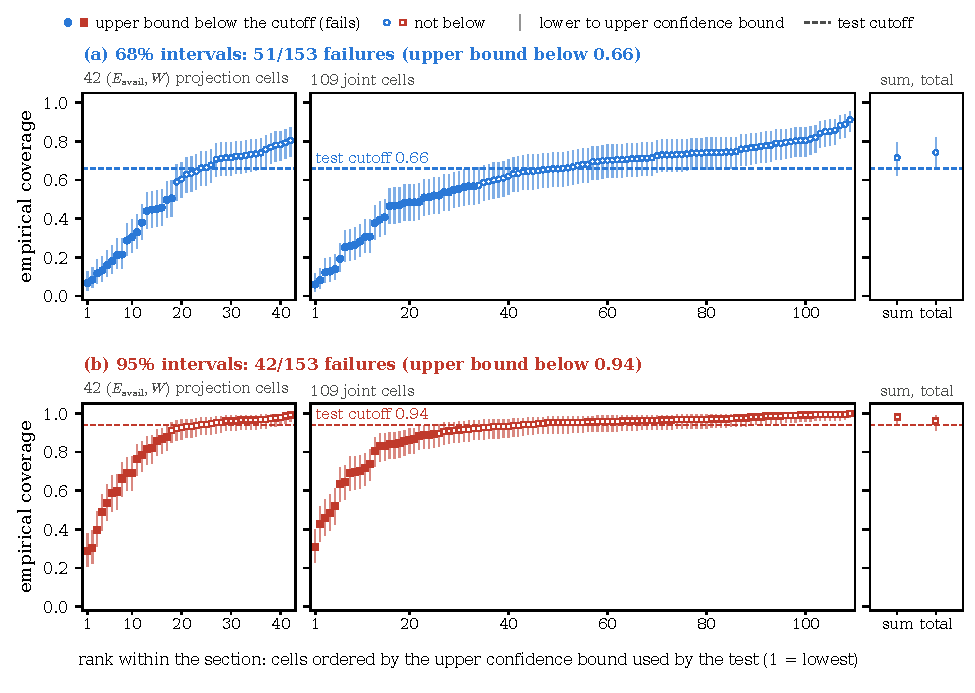
\includegraphics[width=\linewidth]{figures/paper_fig_coverage.pdf}
  \caption{At the reduced signal rate, the deterministic purity control fails the coverage test for 51 of the 153 quantities with the $68\%$ intervals and for 42 with the $95\%$ intervals. The points show the empirical coverage of statistical intervals in 400 pseudo-experiments. Row (a) shows the $68\%$ intervals and row (b) the $95\%$ intervals. Each row shows the 42 $(E_{\mathrm{avail}},W)$ cells, the \jtNcells{} supported joint cells, and the projection sum with the integrated total as separate groups. Within each group, cells are ranked by the upper confidence bound on their coverage. The bars span Clopper--Pearson confidence bounds with a multiplicity correction, and the upper end is the bound the test uses. Filled symbols mark upper bounds below the dashed cutoff, 0.66 for the $68\%$ intervals and 0.94 for the $95\%$ intervals.}
  \label{fig:coverage-5d-paper}
\end{figure}

\subsection{Multidimensional statistical methods}
\label{app:multidimensional-statistics}
\label{app:statmethods-nd}
\label{sec:gbdt-diagnostic-definitions}
\label{sec:unbinned-inference}

We multiply the fine-grid densities by all five bin widths to obtain cell integrals before aggregation. A fixed projection $y=Px$ propagates the covariance as $PCP^{\mathsf T}$, with the integration weights included in $P$ if $x$ is a density. We use the \jtNcells{} supported cells of the three-bin joint grid defined in Appendix~\ref{app:joint-generator-tests}, the \fvval{h2-nsupported} supported cells of the two-bin grid underlying the sixteen-cell result, and the 42 $(E_{\mathrm{avail}},W)$ cells. Support requires at least 1000 expected reconstructed signal events and a selected truth weight of at least 1000 at the data exposure. Applying that rule to the $(E_{\mathrm{avail}},W)$ plane leaves 39 cells for supported-cell summaries.

Repeatability studies summarize the mean and sample standard deviation of $(\widehat f_i-f_{\mathrm{true},i})/f_{\mathrm{true},i}$ for each integral $f$. The truth in this expression can vary with the simulation split, so the spread describes relative residuals for the tested split ensemble. The finite-sample summaries use pointwise Student-$t$ intervals for the mean, $\chi^2$ intervals for the standard deviation, and exact binomial intervals for containment. A fixed-width diagnostic takes its widths from 100 refitted bootstrap replicas of a single nominal pseudo-experiment.

The five-axis purity covariance $C_Z$ uses separate vertical (weight-only), residual, and reselected lateral band sums, plus statistical and training-seed terms. The three band groups are disjoint and cover all 45 bands. The covariance of its \zprojCells-cell $(E_{\mathrm{avail}},W)$ projection is obtained by projecting the five-axis matrix. In joint throws we vary reweightable bands simultaneously using their event weight ratios, interpolating separately toward the positive or negative endpoint according to a standard normal variation, and draw the flux variations. We re-unfold each throw at a fixed training seed. Writing $v_{\mathrm{joint},i}$ for the joint variance about the central value and $v_{\mathrm{vert},i}$ for the vertical-band sum's diagonal, the vertical block is rescaled on both sides by a diagonal matrix with entries
\begin{equation}
 g_i=\sqrt{\max(1,v_{\mathrm{joint},i}/v_{\mathrm{vert},i})},
 \qquad g_i=1\ \text{if }v_{\mathrm{vert},i}=0 .
 \expandafter\let\expandafter\label\csname ltx@label\endcsname
 \label{eq:app-five-axis-inflation}
 \label{eq:zinflation}
\end{equation}
The matching band covariances use universe-mean centering. The joint variance about the central value also includes the squared offset of the joint ensemble mean. The covariance is used as a descriptive scale, with the seed-stability test reported in Sec.~\ref{sec:higher-dimensional-calibration}. The required null bound for that covariance was also unspecified at production.

The paired rounding diagnostic measures the standard deviation of the difference between jittered and unjittered replicas divided by $\sqrt{2}$. We compare this scale from 50 pairs both with the spread from 20 jitters of the base input and with the unperturbed bootstrap spread. Inputs are perturbed within half a single-precision unit in the last place while holding fine-grid membership fixed. The prespecified containment rule requires a median paired-to-base ratio in $[0.7,1.4]$ and bootstrap variance at least as large as the paired estimate in at least $95\%$ of supported cells. This compares variability within the refit procedure.

\subsection{Joint generator tests}
\label{app:joint-generator-tests}

\label{sec:joint5d-design}
\label{sec:joint5d-calibration}
\label{app:joint5d-genmodel}
\label{sec:joint5d-frozen}
\label{sec:joint5d-fwer}


\label{sec:joint5d-kappa}
\label{sec:joint5d-lost}
\label{sec:joint5d-projections}
\label{sec:joint5d-ch}

\paragraph{Hypotheses and metric.} The calibration tests a hybrid null for each of the five predictions in Sec.~\ref{sec:sixteen-cell-generator-comparison}. The null fixes the fine-grid truth integrals to the generator prediction. The shape statistic removes the overall normalization after unfolding. The conditional composition within a fine cell is taken from MINERvA Tune v1 and varied within the specified interaction-model bands. The test statistics use a coarser grid with edges
\begin{align*}
  p_T &: (0,0.55,0.85,4.5)\ \mathrm{GeV}/c , \\
  p_\parallel &: (1.5,3.5,6,60)\ \mathrm{GeV}/c , \\
  E_{\mathrm{avail}} &: (0,0.4,1.5,100)\ \mathrm{GeV} , \\
  q_3 &: (0,1.2,2,100)\ \mathrm{GeV}/c , \\
  W &: (0,1.4,2.2,100)\ \mathrm{GeV} .
\end{align*}
Of the $3^5$ cells, \jtNcells{} satisfy the support rule in Appendix~\ref{app:multidimensional-statistics}. GiBUU uses the \jtNcellsGiBUU{} supported cells with $p_\parallel<6~\mathrm{GeV}/c$. The fine grid is that of Table~\ref{tab:reproducibility-bin-edges}.

For unfolded integrals $F$ and predicted integrals $\mu_G$, the total statistic is $T_{\mathrm{tot}}=(F-\mu_G)^{\mathsf T}\Sigma^{-1}(F-\mu_G)$. The metric $\Sigma=V+\operatorname{diag}[\operatorname{Var}(\mu_G)]$ uses a Ledoit--Wolf shrinkage estimate~\cite{LedoitWolf:2004} $V$ from \jtVn{} MINERvA Tune v1 pilot pseudo-experiments and adds the prediction's diagonal finite-sample variance. For $T_{\mathrm{sh}}$ we use normalized cell fractions, propagate $\Sigma$ through the normalization Jacobian in Eq.~\eqref{eq:app-shape-jacobian}, and drop one redundant fraction. The metric sets the relative weights of the discrepancies. The reference distribution comes from rerunning the estimator with the same fixed metric. It incorporates estimator bias, including retention of the prior, which can shift the null away from a quadratic form centered at zero residual.

\paragraph{Calibration ensemble.} Each draw randomly partitions the simulation into a source half and an unfolding half. In populated fine truth cells we reweight the source signal to $G$. The source weights combine an independently selected flux universe from the \jtFluxUniverses{} available and a uniformly selected universe from each of \jtModelBands{} interaction-model bands. The flux variation changes the source rate for the fixed input cross section. For signal, the interaction-model weights are renormalized within each fine cell. They therefore vary the efficiency and migration through changes in the within-cell composition. Negative weights in two of the bands are clipped. The four weight-based detector bands use equiprobable endpoints. These variations act on the source, which supplies Poisson pseudo-data including MINERvA Tune v1 backgrounds. We unfold with the other half at nominal MINERvA Tune v1 weights, using a disjoint background template and refitting the negative-weight refinement. The test variant uses five OmniFold iterations, selected by a rule based on the largest residual across the simulated truth deformations on the two joint reporting grids. The observed data use the full nominal simulation and background template. No rejection rate has been measured for null pseudo-data processed like the data, which would require an independent simulation sample.
% Search: rejection rate; processed like the data; independent simulation sample @ ddf16f10

Five lateral bands enter through additive shifts $z_b d_b$, with independent standard normal $z_b$ and $d_b$ equal to half the difference between each band's two observed-data endpoint unfolds. This linear surrogate uses inputs estimated on the observed data. Calibration is conditional on those inputs and on the common simulated event pool. An independent Gaussian coefficient propagates the $1.4\%$ normalization. Rounding and generator finite-sample fluctuations are added as Gaussian residuals in each cell. The variance for the latter is the sum of squared generator weights in that cell, in cross-section units. The six conditions on interpreting the tests are listed at the end of this subsection. The available check of the lateral surrogate addresses the symmetry of its endpoints.

\paragraph{Tail probabilities and multiplicity.} At a checkpoint, $k$ of the $B$ completed null draws satisfy $T_{\mathrm{null}}\geq T_{\mathrm{obs}}$, giving the Monte Carlo probability $(k+1)/(B+1)$. We use the largest probability over five separate shifts of the simulated unfolded vectors, $0,D/2,D,+\jtMoneKappa\,\delta_{\mathrm{fine}},-\jtMoneKappa\,\delta_{\mathrm{fine}}$. Here $D$ is the estimated change from the half- to the full-simulation unfolding and $\delta_{\mathrm{fine}}$ is the last measured change under fine-grid refinement. A shift is applied to every draw in its variant before forming the statistic. The envelope tests the listed directions and sizes individually.

The Holm procedure~\cite{Holm:1979} orders the ten probabilities from smallest to largest, with ties in the fixed listing order and total before shape for each generator. At step $i$ the threshold is $c_i=\jtAlpha/(\fpeval{\jtNtests+1}-i)$. Rejection requires the upper endpoint of the two-sided $95\%$ Clopper--Pearson interval~\cite{Clopper:1934} for $k/B$ to be strictly below $c_i$. A lower endpoint above $c_i$ gives nonrejection, and an interval containing $c_i$ leaves the decision undetermined. The first nonrejection or undetermined decision ends the step-down and assigns that status to the remaining tests. Calibration is examined in batches of \jtBatch{}, with the sequential error bound defined through $B=\jtBcap$. The protocol was fixed before the observed statistics and production draws, with data-informed design and budget choices documented in Appendix~\ref{app:choices-after-results}.

For a true null, let $p$ denote the ideal tail probability of the observed statistic. The familywise bound assumes that $p$ is super-uniform under repetition and that, conditional on the data and simulation, the exceedances in fixed seed order are independent Bernoulli draws with probability $p$. Integrating the binomial boundary-crossing probability through \jtBcap{} draws over a uniform $p$ bounds the single-test rejection probability $R(c)$ at threshold $c$. For a specified $p$ the crossing probability can be computed by advancing the binomial count one draw at a time and accumulating the probability removed at each crossing. The crossing probability decreases as $p$ increases, which gives the bound for a super-uniform tail probability. With $m_0$ true nulls, the first true null rejected has threshold at most $\jtAlpha/m_0$. The union bound gives $\max_{1\leq j\leq\jtNtests} j R(\jtAlpha/j)\leq0.8902\times\jtAlpha$, without requiring independence between tests. The maximum over shifts includes the unshifted variant and can only raise its upper endpoint at common $B$. The bound is conditional on the stated assumptions, including outcome-independent loss of calibration draws when using only completed draws.

\paragraph{Sensitivity and interrupted draws.} Sixteen paired unfoldings estimate $D$. Its median absolute size relative to the cell integrals is $0.02\%$--$0.075\%$, and its projection along the null bias direction is at most 0.068 null standard deviations. In a descriptive scan replacing the coefficient \jtMoneKappa{} on $\delta_{\mathrm{fine}}$ with $\kappa$, all ten decisions remain determinate rejections at the sampled values through $\kappa=5.25$. The scan quantifies sensitivity along the measured refinement direction, with the residual below the fine grid unbounded by this check. The fine-grid convergence check has not shown convergence. The matched projection check repeats the calibration on the two $3\times 3$ projections, onto the muon momenta and onto $(E_{\mathrm{avail}},W)$, both with the original shifts projected and with shifts re-estimated on each projection. Its criterion requires both projected probabilities to be at least 0.05 in both evaluations to count a joint rejection as additional discrimination.

The decision samples contain 1365, 1366, \jtBmin{}, \jtBmax{}, and 1351 completed draws for MINERvA Tune v1, GENIE without and with Valencia MEC, NuWro, and GiBUU, respectively. NuWro's shape test has one exceedance and the other tests have zero. Time limits initially removed \jtLostCal{} calibration and \jtLostPow{} power draws. Before recovery, a worst-case assignment of the missing calibration outcomes could change each decision. In particular, the number of lost draws was large compared with the observed exceedance counts and could have affected both the Holm ordering and the interval endpoints. Rerunning the lost seeds found zero additional exceedances for all tested variants. The decisions use the counts at the original sequential stop.

\paragraph{Target correction.} A target-sensitivity check converts the NuWro and GiBUU carbon predictions to hydrocarbon in each fine cell using $x_{\mathrm{CH}}=(12x_{\mathrm C}+ x_{\mathrm H})/13$, with $x_{\mathrm H}$ from the corresponding generator's free-proton sample. We compare the corrected predictions against the original calibration distributions. NuWro's total statistic falls by 3.83 null standard deviations. It would be undetermined at the original Holm threshold of 0.005 and is rejected at the new, last position with threshold 0.05. With the descriptive $\kappa=\jtMoneKappaRobust$ shifts it has $p=0.075$ and is not rejected. The evaluation holds fixed the null distributions calibrated for the original targets, so it is descriptive for the hydrocarbon predictions.

\paragraph{Conditions on the decisions.} Each of the ten decisions in Sec.~\ref{sec:sixteen-cell-generator-comparison} holds under the following six conditions. \phantomsection
% Moved from sec5_multidim.tex (Sec. 5.3, narrative pass 2026-11-22, review item 3); the six items are verbatim and
% the label moved with the list. Sec. 5.3 keeps the familywise rejection, the hybrid scope, the no-uncertainty
% statement and a summary naming the calibration and detector-response conditions.
\label{sec:joint5d-conditions}
\begin{enumerate}
  \item \emph{Subcell composition.} Replacing the below-grid MINERvA Tune v1 composition with the generator's must shift the result by at most twice the last measured refinement change along that direction.
  \item \emph{Detector response.} The specified detector variations must be adequate despite the absence of a dedicated calorimetric recoil-energy-scale variation.
  \item \emph{Interaction model.} The \jtModelBands{} bands must describe within-cell composition and its effects on efficiency and migration.
  \item \emph{Calibration.} Tail probabilities from half-sample pseudo-experiments must apply to the full-sample data unfolding, conditional on the available simulation, with independent exceedances. No rejection rate has been measured for null pseudo-data processed like the data, and the lost pseudo-experiments have not been shown to be lost independently of their outcomes.
  \item \emph{Neutrino-energy range.} The samples must describe migrations into the test domain, including for GiBUU with $E_\nu<\fvval{cmodel-gibuu-enu}~\mathrm{GeV}$.
  \item \emph{Finite generator samples.} Independent Gaussian residuals must adequately describe finite-sample errors in the predictions.
\end{enumerate}

\clearpage
\subsection{Validation-test inventory}
\label{app:validation-inventory}

\begingroup \small
\setlength{\LTcapwidth}{\textwidth}
\setlength{\LTpre}{4pt}
\setlength{\LTpost}{0pt}
% xltabular creates the caption anchor when the table starts. Suppress hyperref's extra anchor from stepping the same table counter.
\makeatletter
\ifdefined\XLT@refstepcounter \ifdefined\H@refstepcounter
    \let\XLT@refstepcounter\H@refstepcounter
  \fi
\fi
\makeatother
\begin{xltabular}{\textwidth}{@{}
  >{\footnotesize\RaggedRight\arraybackslash\hsize=1.0\hsize}X >{\footnotesize\RaggedRight\arraybackslash\hsize=0.85\hsize}X >{\footnotesize\RaggedRight\arraybackslash\hsize=1.15\hsize}X >{\footnotesize\RaggedRight\arraybackslash\hsize=1.0\hsize}X@{}}
  \caption{Validation tests and scoring rules for the estimators in Table~\ref{tab:estimators}. A prespecified criterion was recorded before its outcome was read. Appendix~\ref{app:choices-after-results} gives the data-informed choices.}
  \label{tab:validation-inventory}\label{tab:test-index}\label{tab:closure-map}\\
  \toprule Test & Estimator or sample & Criterion and status & Outcome and scope \\
  \midrule \endfirsthead \multicolumn{4}{@{}l}{\tablename~\thetable\ (continued)} \\
  \toprule Test & Estimator or sample & Criterion and status & Outcome and scope \\
  \midrule \endhead \bottomrule \endfoot \multicolumn{4}{@{}l}{\textit{Two-dimensional benchmark and checks across dimensions}} \\
  \addlinespace[1.5pt] Ordinary closure & Simulated reconstruction unfolded to its own truth & Descriptive bookkeeping check & Recovers the input in an identity test. \\
  \addlinespace[1.5pt] Event matching and iteration stability & Truth and reconstructed event records and exact-split 2D cross-check & Event-list completeness and five-versus-ten-iteration comparison & Truth-only entries are retained. The exact-split total changes by at most $0.026\%$ between five and ten iterations. \\
  \addlinespace[1.5pt] Published 2D result & \estTwoD{}, purity baseline, and exact-split cross-check on 205 bins & Descriptive, owing to shared data and systematics & Integral agrees to about $1\%$. A correlated shape difference remains. \\
  \addlinespace[1.5pt] Binned IBU benchmark in 2D & Ten-iteration binned IBU and \estTwoD{} with shared inputs & Null from \fvval{c2c1-nrep} paired replicas & $T=\fvval{c2c1-T}$ exceeds the null 95th percentile of \fvval{c2c1-q95}. \\
  \addlinespace[1.5pt] Run-period contribution to the published comparison & Separate unfolds of the three groups & Prespecified comparison in published-covariance eigenmodes & The step fails to explain the discrepancy in the best-determined directions at the test sensitivity. \\
  \addlinespace[1.5pt] \hypertarget{validation-2d-closure}{}Gaussian $p_T$ and tilted $p_\parallel$ truth & 2D purity baseline, signal only & Descriptive $1.5\%$ residual threshold & Residuals $0.046\%$ and $0.013\%$. \\
  \addlinespace[1.5pt] Injected $17.2\%$ Gaussian feature & 2D purity baseline, signal only & Descriptive recovery check of Ref.~\cite{Canelli:2025guide} & $1.69\%$ residual, or 0.098 of the injection. \\
  \addlinespace[1.5pt] Alternative axial-mass and flux universes & Signal-only 2D purity baseline with accepted truth extrapolated to the reporting domain & Descriptive $2\%$ residual threshold & Residuals $0.068\%$ and $0.376\%$ against the constructed references. \\
  \addlinespace[1.5pt] \hypertarget{validation-2d-response}{}Hidden $\Delta p_T$ deformation & 2D purity baseline, fixed truth & Descriptive $3\%$ residual threshold & Leakage scales with amplitude. The largest arm gives $3.43\%$. \\
  \addlinespace[1.5pt] Background-inclusive closure & 2D purity and refined subtraction on 20 paired nominal-truth draws & Descriptive comparison at a common statistical scale & Differences exceed $1\sigma$ in 14 bins. The refined result is closer to truth in those bins. \\
  \addlinespace[1.5pt] Same-ensemble pull check & 200 two-dimensional closure unfolds & Descriptive because the scale is estimated on the scored draws & $\pullFrac\%$ of pulls within one standard deviation. \\
  \addlinespace[1.5pt] Fixed-truth statistical coverage & Earlier 2D band with a completeness correction & Prespecified one- and two-standard-deviation windows & Coverage is \covTwoDCOne{} and \covTwoDCTwo{}, respectively. The two-standard-deviation band fails. \\
  \addlinespace[1.5pt] \hypertarget{validation-2d-joint-coverage}{}Held-out-tune closure & Rebuilt 2D covariance at two GENIE v3 tunes, including prior-shape term and omitting run-period term & Prespecified joint minima of \lrval{cov2d-ar23-kjoint} and \lrval{cov2d-g18-kjoint} of \lrval{cov2d-ntoys} at the two tunes & Joint undercoverage at both tunes. Bias drives the flagged bins. \\
  \addlinespace[1.5pt] Classifier two-sample diagnostic & Reconstructed data and reweighted simulation & Descriptive because training and evaluation share the sample & Area under the ROC curve falls from about 0.535 to 0.501. \\
  \midrule \multicolumn{4}{@{}l}{\textit{Higher-dimensional recovery and estimator dependence}} \\
  \addlinespace[1.5pt] \hypertarget{validation-nd-bumps}{}$E_{\mathrm{avail}}$ and $q_3$ bumps & 3D and 4D purity baseline, signal only & Descriptive, with no prespecified thresholds & Marginal residuals $1.84\%$ and at most $1.1\%$. \\
  \addlinespace[1.5pt] \hypertarget{validation-nd-w-bump}{}$W$ bump at the $\Delta$ peak & 5D purity baseline, signal only & Prespecified marginal residual-to-injection limit of 0.20 & Ratio 0.180 passes. Joint peak-column cells are up to $9.4\%$ low. \\
  \addlinespace[1.5pt] Background-inclusive closure & 5D deterministic purity control, low-capacity refinement, and sixteen-cell estimator at nominal truth & Descriptive, with no common prespecified criterion & Negative weights reduce the high-$W$ bias. The sixteen-cell estimator gives a pooled pull width of 1.02. \\
  \addlinespace[1.5pt] Generator-sized $E_{\mathrm{avail}}$ change & Low-capacity refinement with backgrounds and a signal-only repeat & Prespecified recovery requirement & Fails with a median $(E_{\mathrm{avail}},W)$ residual of $9.7\%$ and a maximum of $74\%$. \\
  \addlinespace[1.5pt] Withheld generator-derived shapes & Sixteen-cell estimator, scored on $(E_{\mathrm{avail}},W)$ integrals & Descriptive recovery scores & Median recovered fractions $\fvval{rec-w-fmed-lo}\%$--$\fvval{rec-w-fmed-hi}\%$. Some cells move opposite to the injection. \\
  \addlinespace[1.5pt] Hidden $q_3$ deformation & Low-capacity refinement at fixed $(E_{\mathrm{avail}},W)$ truth, with a signal-only repeat & Descriptive response to amplitude 0.3 & $(E_{\mathrm{avail}},W)$ cells shift by up to $37\%$. \\
  \addlinespace[1.5pt] Shifted recoil response & Sixteen-cell estimator at nominal truth with signal only & Descriptive, with no prespecified threshold & Largest change is $\fvval{ct3b-species-max}\sigma$ for deposit variations and $\fvval{ct3b-w2b-max}\sigma$ for the whole-recoil scale. \\
  \addlinespace[1.5pt] Reporting-resolution precision & Sixteen-cell estimator and its admissible settings on two joint grids and the $(E_{\mathrm{avail}},W)$ plane & Prespecified width, model-sensitivity, and recovery targets & All three grids miss the targets. \\
  \addlinespace[1.5pt] \hypertarget{validation-sixteen-bias}{}Fake-data bias & Sixteen-cell estimator at \fvval{f0b-all-truths} truths, with separate held-out-tune controls & Prespecified $p<\fvval{trig-p}$ or any $|z|>\fvval{trig-z}$ for flagging & GiBUU hybrid flagged with $C_{\mathrm{rep}}$. Under the earlier $C_e$, the $q_3$ tilt was also flagged. Both held-out controls stay within the criteria. \\
  \addlinespace[1.5pt] Prior retention and algorithm settings & Sixteen-cell estimator at the two truths flagged under $C_e$ and a binned IBU control & Prespecified change of \fvval{prr-floor} in retained fraction & Both flags persist across the refined settings under $C_e$, and the GiBUU hybrid's under $C_{\mathrm{rep}}$. Under $C_e$, binned IBU clears the tilt flag. \\
  \addlinespace[1.5pt] Classifier family & 3D purity baseline with trees or a multilayer perceptron & Descriptive, with no prespecified agreement threshold & Median projection differences of $0.7\%$--$1.4\%$. \\
  \addlinespace[1.5pt] Binned IBU on data & Sixteen-cell estimator and five-iteration IBU on common inputs & Prespecified comparison with matched-difference null & $T=\lrval{rg1-T}$ exceeds the calibrated \fpeval{100*\lrval{rg1-lev1}}th and \fpeval{100*\lrval{rg1-lev2}}th percentiles. \\
  \midrule \multicolumn{4}{@{}l}{\textit{Higher-dimensional coverage, stability, and generator tests}} \\
  \addlinespace[1.5pt] \hypertarget{validation-purity-coverage}{}End-to-end statistical coverage & Deterministic 5D purity control on 153 integrals & Prespecified minimum upper confidence bounds of 0.66 and 0.94 for $68\%$ and $95\%$ intervals, respectively & Fails at nominal and reduced signal rates. \\
  \addlinespace[1.5pt] First sixteen-cell coverage test and staged test & Covariance at two held-out tunes & Prespecified entry checks & The first stopped at an entry gate before any coverage pseudo-experiment ran; the staged redesign stopped at its first stage. \\
  \addlinespace[1.5pt] \hypertarget{validation-sixteen-coverage}{}Sixteen-cell held-out-tune closure & $C_{\mathrm{total}}$ at both held-out tunes & Joint minimum of \fvval{ll5d-kjoint-all} in \fvval{ll5d-ntoys} draws. Descriptive because part of the procedure was fixed after an early stop. & Joint undercoverage in both band variants at both tunes. \\
  \addlinespace[1.5pt] \hypertarget{validation-sixteen-rounding}{}Rounding-level stability & Sixteen-cell estimator on data, with low-capacity refinement and ensemble-average controls & Prespecified median and maximum shift tolerances of $\fvval{ens1-bar-median}\sigma$ and $\fvval{ens1-bar-max}\sigma$ & Fails on data. Averaging passes on tested pseudo-data but worsens GiBUU-like closure. \\
  \addlinespace[1.5pt] Rounding variability in the bootstrap & Pairs with the same Poisson draws, with and without input rounding perturbations & Prespecified paired-to-base spread and variance criteria & Meets containment for the tested estimator and supported cells. \\
  \addlinespace[1.5pt] Seed stability of $C_Z$ & Companion exploratory purity covariance builds & Prespecified $\sprojBound\%$ projection tolerance & Largest shift is $\sprojMeasured\%$. Five bands were held fixed. \\
  \addlinespace[1.5pt] Muon-quadrant sums & Sixteen-cell and 2D results, with a descriptive comparison to 3D central values & Prespecified covariance and correlation-scan rule for 2D & Coarse muon projections agree over the full scan. \\
  \addlinespace[1.5pt] Joint generator tests & Variant of the \estMultiD{} on \jtNcells{} cells (\jtNcellsGiBUU{} for GiBUU) & Prespecified protocol with data-informed elements and familywise level \jtAlpha{} & All ten hybrid nulls rejected under the stated conditions. \\
  \addlinespace[1.5pt] Matched coarse projections & Same joint-test inputs projected onto the two $3\times3$ planes & Criterion fixed after the joint results and before the projections ran & No joint test meets the criterion for additional discrimination. \\
  \addlinespace[1.5pt] Joint-test sensitivity checks & Shift scan, recovered draws, and CH target correction & Descriptive evaluations outside the joint decision rule & Zero recovered exceedances. NuWro total is sensitive to the target and shift size. \\
\end{xltabular}
\endgroup

% PASS2: Literal numerical values with no matching source macro for the same quantity:
% - Covariance and inversion: 300 statistical bootstraps; 20 replicas per seed, N=5 and 1/20; 100 PPFX universes in the 2D sweep; 187 universes in 44 bands with 43 retained; 0.014 target normalization; the 10^-12 ridge, 10^-15 SVD and 10^-12/10^-10 spectral cuts; ranks 138, 205 and 198; condition number 7.95 x 10^11; 21.96 for the direct inverse; generic 16 and 15 dimensions.
% - Comparison and closure: 205 bins, the 14 x 16 grid and 204 shape directions; truth injection 0.2/0.4/0.1 and tilt 0.1/5; hidden-variable center and width 0.10/0.05 and amplitudes 0.05/0.10/0.30; bias-test rank 16 and cuts 0.01 and 2; the statistical band-to-scatter bounds 0.9 and 1.1; 200 same-ensemble replicas and the Gaussian reference 0.6827.
% - Multidimensional methods: 42 projection cells (39 with support), support of 1000 events/weight, 100 diagnostic refits, 400 draws per truth and 153 integrals for end-to-end coverage, 0.66/0.94 at 68%/95%, rate tilt 0.2 and 100 GeV, 45 covariance bands, 50 rounding pairs and 20 base jitters, and the paired criteria [0.7,1.4] and 95%.
% - Joint tests: coarse grid edges and GiBUU's 6 GeV/c cut, 1.4% normalization, the 95% interval, 0.8902 bound, paired shift 0.02%--0.075% and 0.068 SD, kappa scan through 5.25, projection cutoff 0.05, counts 1365/1366/1351, CH coefficients 12 and 13, and the NuWro values 3.83, 0.005, 0.05, 0.075.
% - Inventory: 205 bins and about 1% integral agreement, the 2D IBU 95th percentile, truth closure 1.5%/0.046%/0.013% and 17.2%/1.69%/0.098, alternative-universe 2%/0.068%/0.376%, hidden resolution 3%/3.43%, background closure 20 draws/1 sigma/14 bins, 200 same-ensemble draws, ROC areas 0.535/0.501, marginal bumps 1.84%/1.1%/0.20/0.180/9.4%, pooled width 1.02, residuals 9.7%/74%, hidden q_3 amplitude 0.3 and shift 37%, bias criteria 0.01 and 2, classifier differences 0.7%--1.4%, and 153 coverage integrals. Mathematical and layout constants are literal.
% - The supplied excerpts do not print every table value retained in pass 1. No corresponding source macro was found for the ROC areas, 2D background closure counts, pooled width 1.02 or the classifier-family differences. Labels and placement:
% - eq:blocksum and eq:diffcov belong with eq:muon-covariance-block-sum and eq:muon-difference-covariance, respectively, in the rewritten main text. eq:systblocksum has no numbered counterpart in this rewrite.
% - tab:variance-sources, tab:band-medians, tab:joint5d-genmodel, tab:joint5d and fig:joint5d-nulls have no standalone object in the current Appendix A. There was no cropped or placeholder figure here to replace.
% - sec:part-q3 and the sec_systematics.tex section labels belong to the main text. The sec_systematics.tex floats fig:bootstrap, fig:uqbands and tab:pl-added were not retained here.
% - sec:joint5d-power, sec:joint5d-response and sec:joint5d-reading have no standalone counterpart in the current Appendix A.
% - For references in this file, all targets are present locally or in inputs2/new-labels.md.
